\chapter{Capture, SINR and Successive Interference Cancellation}
\label{ch:sic}

\begin{defbox}[In this chapter you will learn]
\begin{itemize}
 \item the \emph{physical} (SINR-threshold) model of a collision and the \emph{capture effect};
 \item the principle of \emph{successive interference cancellation} (SIC), why it works best when received powers differ, and how imperfect cancellation changes the SINR sequence;
 \item exactly how Amber groups, resolves and logs colliding packets, step by step;
 \item three behaviours of that pipeline that differ from textbook expectations, each verified by experiment, including a measured \emph{SIC on/off} ablation.
\end{itemize}
\end{defbox}

\section{From ``collision'' to SINR}
\label{sec:physmodel}

Chapter~\ref{ch:aloha} treated a collision as a binary event: if two packets share a
slot, both are lost. This is the \emph{protocol model}. Real receivers are more
forgiving. A packet can be decoded despite overlapping with another if it is
\emph{strong enough} relative to everything else. This is the \emph{physical model}: packet $i$ is
decoded if its signal-to-interference-plus-noise ratio
\begin{equation}
 \gamma_i=\frac{P_i}{\sum_{j\ne i}P_j+N}\ \ge\ \gamma_{\mathrm{req}}.
\label{eq:sinrdef}
\end{equation}
The threshold $\gamma_{\mathrm{req}}$ is a single number that stands in for the modulation, coding and
receiver design (Amber's default in the base station is $3$~dB).

\paragraph{The capture effect.}
When two packets collide and one is much stronger, the receiver locks onto it and ignores the other. Roberts called this
\emph{capture} \citep{roberts1975}. For two packets of power $P_1\ge P_2$ and negligible noise, capture requires
\[
 \frac{P_1}{P_2}\ge\gamma_{\mathrm{req}}
 \quad\Longleftrightarrow\quad
 (P_1-P_2)_{\mathrm{dB}}\ge(\gamma_{\mathrm{req}})_{\mathrm{dB}}.
\]
Noise changes this when the weaker packets are near the noise floor, as Figure~\ref{fig:sinrgap} shows: a strong
pair ($-60$~dBm) is interference-limited and the SINR grows without bound with the gap; a weak pair ($-80$~dBm)
is noise-limited and saturates at about $8$~dB no matter how small the interferer.

\begin{figure}[t]
\centering
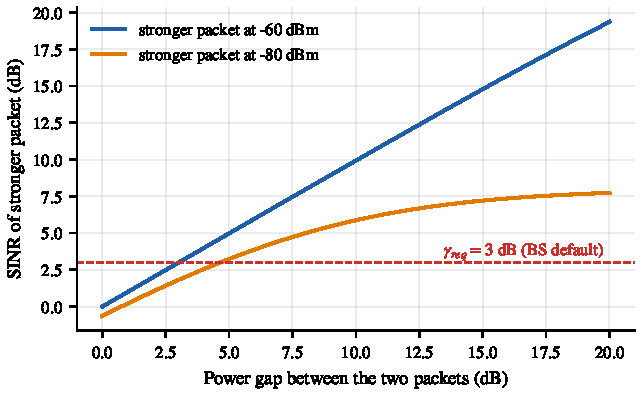
\includegraphics[width=0.62\linewidth]{fig_sinr_vs_gap}
\caption{SINR of the stronger of two colliding packets against the power gap, for thermal noise $\SI{-88}{dBm}$. At $-60$~dBm the curve is interference-limited; at $-80$~dBm it saturates because noise dominates. The dashed line is Amber's default requirement of $3$~dB.}
\label{fig:sinrgap}
\end{figure}

\paragraph{Why capture matters for backscatter.}
In Chapter~\ref{ch:backscatter} we saw that the uplink loses $2\times10\,n\log_{10}d$~dB: for a pair of
nodes whose distances differ by a factor of $2$, the received powers differ by
$2\cdot22\log_{10}2=\SI{13.2}{dB}$ below the UMa breakpoint and $2\cdot40\log_{10}2=\SI{24.1}{dB}$ beyond it. This
\emph{near--far diversity} makes capture frequent: random placement itself supplies power differences.

\section{Successive interference cancellation}
\label{sec:sictheory}

\subsection{The principle}

Capture decodes the strongest packet and discards the rest. But the others
may be perfectly decodable \emph{once the strongest is out of the way}. SIC makes this explicit \citep{tse2005,cover2006}:
\begin{enumerate}
 \item sort the received signals by power;
 \item decode the strongest, treating all others (and noise) as interference;
 \item if decoding succeeded, \emph{reconstruct and subtract} that signal from the received waveform;
 \item repeat on the remainder; stop at the first failure.
\end{enumerate}
In information theory, SIC with ideal cancellation achieves the corner points of the multiple-access capacity region,
which is why it is considered the receiver of choice in non-orthogonal multiple access (NOMA).

\subsection{The SINR sequence}

Let the powers sorted in decreasing order be $P_{(1)}\ge P_{(2)}\ge\dots\ge P_{(m)}$ and let $\varepsilon\in[0,1]$ be the fraction of an
already-decoded signal that is \emph{not} removed ($\varepsilon=0$: perfect cancellation). When decoding the $k$-th strongest,
\begin{equation}
 \gamma_{(k)}=\frac{P_{(k)}}{\displaystyle\sum_{j>k}P_{(j)}+\varepsilon\sum_{j<k}P_{(j)}+N}.
\label{eq:sicsinr}
\end{equation}
With perfect cancellation only \emph{weaker} packets interfere. A useful design rule follows: if successive powers
decrease by a constant ratio $\rho$ and noise is negligible, the SINR of every stage is
$1/(\rho^{-1}+\rho^{-2}+\cdots)=\rho-1$, so SIC decodes all packets iff $\rho\ge1+\gamma_{\mathrm{req}}$.
\emph{Each packet must be stronger than the sum of all weaker ones by the decoding threshold.}
For $\gamma_{\mathrm{req}}=3$~dB this means $\rho\ge3$ ($4.8$~dB) between neighbours.

\begin{figure}[t]
\centering
\begin{tikzpicture}[x=1cm,y=1cm,scale=0.92]
 \def\u{4.0}
 % powers (linear, relative to P1): 1, 0.316, 0.1, 0.0016
 % ---- column 1: all packets present
 \begin{scope}[shift={(0,0)}]
  \draw[fill=agrey!50] (0,0) rectangle (1.4,0.02);
  \draw[fill=agreen!70] (0,0.02) rectangle (1.4,0.42);
  \draw[fill=aorange!70] (0,0.42) rectangle (1.4,1.69);
  \draw[fill=ablue!75,line width=1.4pt] (0,1.69) rectangle (1.4,5.69);
  \node[white,font=\sffamily\small] at (0.7,3.7) {$P_1$};
  \node[font=\sffamily\scriptsize] at (0.7,1.05) {$P_2$};
  \node[font=\sffamily\scriptsize] at (0.7,0.22) {$P_3$};
  \draw[decorate,decoration={brace,amplitude=4pt}] (1.5,1.69) -- (1.5,0) node[midway,right=5pt,font=\sffamily\scriptsize,align=left] {interference\\$P_2{+}P_3{+}N$};
  \node[font=\sffamily\scriptsize,align=center] at (0.7,-0.75) {\textbf{step 1}: decode $P_1$\\ $\gamma_1=3.79$~dB $\ge3$ \checkmark};
 \end{scope}
 % ---- column 2: P1 removed
 \begin{scope}[shift={(5.6,0)}]
  \draw[fill=agrey!50] (0,0) rectangle (1.4,0.02);
  \draw[fill=agreen!70] (0,0.02) rectangle (1.4,0.42);
  \draw[fill=aorange!70,line width=1.4pt] (0,0.42) rectangle (1.4,1.69);
  \draw[dashed,agrey] (0,1.69) rectangle (1.4,5.69);
  \node[agrey,font=\sffamily\scriptsize,align=center] at (0.7,3.7) {$P_1$ decoded\\and subtracted};
  \node[font=\sffamily\scriptsize] at (0.7,1.05) {$P_2$};
  \node[font=\sffamily\scriptsize] at (0.7,0.22) {$P_3$};
  \draw[decorate,decoration={brace,amplitude=3pt}] (1.5,0.42) -- (1.5,0) node[midway,right=5pt,font=\sffamily\scriptsize,align=left] {$P_3{+}N$};
  \node[font=\sffamily\scriptsize,align=center] at (0.7,-0.75) {\textbf{step 2}: decode $P_2$\\ $\gamma_2=4.93$~dB \checkmark};
 \end{scope}
 % ---- column 3
 \begin{scope}[shift={(11.2,0)}]
  \draw[fill=agrey!50] (0,0) rectangle (1.4,0.02);
  \draw[fill=agreen!70,line width=1.4pt] (0,0.02) rectangle (1.4,0.42);
  \draw[dashed,agrey] (0,0.42) rectangle (1.4,1.69);
  \draw[dashed,agrey] (0,1.69) rectangle (1.4,5.69);
  \node[font=\sffamily\scriptsize] at (0.7,0.22) {$P_3$};
  \draw[decorate,decoration={brace,amplitude=2pt}] (1.5,0.02) -- (1.5,0) node[midway,right=3pt,font=\sffamily\scriptsize] {$N$};
  \node[font=\sffamily\scriptsize,align=center] at (0.7,-0.75) {\textbf{step 3}: decode $P_3$\\ $\gamma_3=17.98$~dB \checkmark};
 \end{scope}
\end{tikzpicture}
\caption{SIC on three colliding packets at $-60$, $-65$ and $-70$~dBm with a $\SI{-88}{dBm}$ noise floor and $\gamma_{\mathrm{req}}=3$~dB. Bar heights are \emph{linear} power. Without cancellation only the strongest would be decoded (capture); with SIC all three are.}
\label{fig:sicsteps}
\end{figure}

\begin{example}[Three packets, with and without SIC]
Powers $-60,-65,-70$~dBm, i.e.\ $1.00,\,0.316,\,0.100$~nW, noise $1.59$~pW. Step~1: $\gamma_1=1/(0.316+0.100+0.0016)=2.39=\SI{3.79}{dB}\ge3$, decoded.
After removal, step~2: $\gamma_2=0.316/(0.100+0.0016)=3.11=\SI{4.93}{dB}$, decoded. Step~3: $\gamma_3=0.100/0.0016=62.8=\SI{17.98}{dB}$, decoded. All three succeed;
capture alone would deliver only the first. If the packets were $-60$ and $-63$~dBm, $\gamma_1=\SI{2.99}{dB}<3$: \emph{nothing} is decoded, a razor-edge illustrating how sharp the threshold model is.
With $10\%$ residual ($\varepsilon=0.1$) step~2 becomes $\gamma_2=0.316/(0.100+0.0016+0.1\cdot1.0)=1.57=\SI{1.96}{dB}<3$: the second packet is \emph{lost}. SIC is very sensitive to cancellation quality.
\end{example}

\section{How Amber resolves collisions}
\label{sec:ambercollisions}

The base station resolves collisions at the \emph{end of each RX window}. Algorithm~\ref{alg:rxbuffer} states the procedure in plain steps; we then explain each design choice.

\begin{algorithm}[t]
\caption{Processing of one RX window (\code{BSBehavior._process_rx_buffer})}
\label{alg:rxbuffer}
\begin{algorithmic}[1]
\Require buffer $\mathcal B$ of arrivals $(t_i,\mathrm{node}_i,P_i,\mathrm{sector}_i,c_i)$ collected during this window; noise $N$; $\gamma_{\mathrm{req}}$
\State group the arrivals by subcarrier shift $c$
\For{each shift group $\mathcal G$}
  \State sort $\mathcal G$ by arrival time; $\mathrm{used}\gets\emptyset$; $\mathrm{coll}\gets[\,]$
  \For{each packet $i$ in time order, $i\notin\mathrm{used}$}
     \State $\mathcal C\gets\{i\}\cup\{j\notin\mathrm{used},\,j\ne i:\ |t_i-t_j|\le\SI{5}{ms}\}$
     \State \textbf{if} $|\mathcal C|>1$ \textbf{then} append $\mathcal C$ to $\mathrm{coll}$ \textbf{end if}; \quad $\mathrm{used}\gets\mathrm{used}\cup\mathcal C$
  \EndFor
  \For{each collision group $\mathcal C$ in $\mathrm{coll}$}
     \State $\mathrm{dec}\gets$ \Call{SIC}{powers of $\mathcal C$, $N$, $\gamma_{\mathrm{req}}$}
     \State \textbf{if} SIC is disabled \textbf{then} $\mathrm{dec}\gets$ first element of $\mathrm{dec}$ \textbf{end if} \Comment{capture only}
  \EndFor
  \For{each packet $p\in\mathcal G$}
     \State $\mathrm{collided}\gets(p\ \text{is in a collision group})\wedge(p\notin\mathrm{dec})$
     \State \textbf{skip} $p$ if its sector index is invalid or $P_p<$ sensitivity of its sector
     \State log \code{RxPacket}$(\dots,\mathrm{collided})$; update counters
     \State \textbf{if not} collided \textbf{then} record node as decoded; queue an ACK if new \textbf{end if}
  \EndFor
\EndFor
\end{algorithmic}
\end{algorithm}

\begin{algorithm}[t]
\caption{SIC as implemented (\code{packet_analysis.apply_sic})}
\label{alg:sic}
\begin{algorithmic}[1]
\Require powers $P_i$ (W), noise $N$, $\gamma_{\mathrm{req}}$, cancellation factor $\kappa$
\State $R_i\gets P_i$; $\mathrm{cand}\gets$ all packets; $\mathrm{dec}\gets[\,]$
\While{$\mathrm{cand}\ne\emptyset$}
  \State $k\gets\arg\max_{i\in\mathrm{cand}}R_i$
  \State $\gamma_k\gets R_k/\big(\sum_{j\in\mathrm{cand},j\ne k}R_j+N\big)$
  \If{$\gamma_k\ge\gamma_{\mathrm{req}}$}
     \State append $k$ to $\mathrm{dec}$; remove $k$ from $\mathrm{cand}$; $R_k\gets(1-\kappa)P_k$ \Comment{residual stored, but never summed again}
  \Else \ \textbf{break}
  \EndIf
\EndWhile
\State \Return $\mathrm{dec}$
\end{algorithmic}
\end{algorithm}

\paragraph{Design choice 1: the buffer is per RX window.}
Each \codew{("rx", d, id)} schedule entry is a separate window, and the buffer is cleared at its start. Consequently \emph{packets in different windows never collide}: a window is one \emph{slot} in the sense of Chapter~\ref{ch:aloha}.

\paragraph{Design choice 2: collision means time-proximity, not overlap.}
A simulated backscatter packet has no duration in the buffer---it is a point event at the instant of transmission. The simulator
therefore declares two packets to collide if they are within $\SI{5}{ms}$ of each other (the \codew{collision_window_ms} argument).
Within one slot of \SIrange{8}{15}{ms}, two nodes that choose the same slot but start $\SI{6}{ms}$ apart (for instance
because one was still in its \emph{processing} state when the slot opened) do \emph{not} collide.

\paragraph{Design choice 3: the group is built greedily.}
For each unused packet $i$, the group consists of $i$ and \emph{all unused packets within $5$~ms of $i$}. This is a greedy neighbourhood, not transitive clustering.
We tested arrivals at $10,14,18$~ms: packets at $10$ and $14$ form a group and collide, but the packet at $18$ ($4$~ms from the second one, $8$~ms from the first) is \emph{not} in it and is decoded
as a lone packet. Exercise~\ref{ex:greedy} asks you to find the logic.

\paragraph{Design choice 4: capture-only without SIC.}
With SIC off the base station runs the same routine with $\kappa=0$ and keeps only the first decoded packet (the strongest, if its SINR
passes). So ``SIC off'' means \emph{capture only}, ``SIC on'' means \emph{every packet that passes the successive test is kept}.

\paragraph{Design choice 5: subcarriers are perfectly orthogonal.}
Packets with different \codew{subcarrier_shift} values are placed in different groups and \emph{cannot} collide, as discussed in Chapter~\ref{ch:backscatter}.

\begin{reality}[Three things the pipeline does that you might not expect]
\textbf{(1) The cancellation factor is inert.} The \code{apply_sic} docstring explains that $\kappa=0.9$ leaves $10\%$ of a decoded signal as residual interference. In the
implementation (Algorithm~\ref{alg:sic}, line~7) the residual $(1-\kappa)P_k$ is stored, but the decoded packet has just been removed from the candidate set, and interference is summed
only over candidates; the residual is never used. We confirmed this by running \code{apply_sic} on several power sets with $\kappa\in\{0,0.5,0.9,0.99,1\}$: the decoded sets were \emph{identical in every case}. Amber's ``SIC'' is therefore
\emph{perfect} cancellation; imperfect cancellation (Eq.~\eqref{eq:sicsinr} with $\varepsilon>0$) is not simulated. The fix would be a one-line change
that adds the residuals of already-decoded packets to the interference sum.

\textbf{(2) A lone packet bypasses the SNR test.} The noise power enters \emph{only} the SINR computation of colliding groups. A single packet that passes the sector's sensitivity gate is logged as decoded regardless of its SNR. We injected a packet at $\SI{-105}{dBm}$
(SNR $=-17$~dB against $\SI{-88}{dBm}$ of noise) and it was decoded.

\textbf{(3) Sub-sensitivity packets still interfere.} The sensitivity filter is applied \emph{after} the SIC decision, so a packet below the sector's sensitivity is dropped from the log but still counted as an interferer for the packets around it.
\end{reality}

\section{Does SIC matter? A controlled experiment}
\label{sec:sicexperiment}

The two shipped broadcast demos differ in \emph{six} ways at once: \code{enable_sic}, capacitance ($300\to\SI{200}{\micro F}$), RX slot length
($10\to\SI{15}{ms}$), slots per frame ($2\to3$), sector beamwidth ($65^\circ\to30^\circ$) and sector sensitivity ($-100\to\SI{-80}{dBm}$). Their results therefore cannot isolate the effect of SIC. We rebuilt the scenario with a single function
and varied the factors one at a time over ten random seeds (script \file{textbook/code/sic_ablation.py}). Table~\ref{tab:sicablation} shows the result.

\begin{table}[t]
\centering
\small
\caption{Delivery error rate (DER $=1-\text{decoded}/\text{sent}$) and throughput of the 3-node broadcast scenario over $\SI{20}{s}$, mean over $10$ seeds (standard deviation of DER in brackets).}
\label{tab:sicablation}
\renewcommand{\arraystretch}{1.1}
\begin{tabular}{@{}lrrr@{}}
\toprule
Configuration & SIC & DER & Throughput (pkt/s)\\
\midrule
Broadcast demo parameters & off & $2.57\%$ ($0.85$) & $6.06$\\
Broadcast demo parameters & on & $0.00\%$ ($0.00$) & $6.22$\\
SIC-demo parameters & off & $2.89\%$ ($1.61$) & $6.41$\\
SIC-demo parameters & on & $0.00\%$ ($0.00$) & $6.60$\\
\midrule
\multicolumn{4}{@{}l}{\emph{One factor changed from the broadcast demo (SIC off)}}\\
Capacitance $\SI{200}{\micro F}$ & off & $2.36\%$ ($0.71$) & $6.80$\\
RX slot $\SI{15}{ms}$ & off & $2.55\%$ ($1.18$) & $5.93$\\
$3$ slots & off & $2.12\%$ ($1.16$) & $5.99$\\
Beamwidth $30^\circ$ & off & $2.57\%$ ($0.85$) & $6.06$\\
Sector sensitivity $\SI{-80}{dBm}$ & off & $2.57\%$ ($0.85$) & $6.06$\\
\bottomrule
\end{tabular}
\end{table}

The conclusions are clean. (i) Enabling SIC removes \emph{all} delivery errors, from $\approx2.6$--$2.9\%$ to $0.00\%$, in both parameter sets. (ii) None of the other factors changes DER meaningfully; beamwidth and sector
sensitivity have \emph{exactly} the same value because all three nodes sit on the sector's boresight and far above $\SI{-80}{dBm}$. (iii) SIC raises throughput slightly
($\approx+2.6\%$) simply because the lost packets are recovered. The improvement shown by the shipped SIC demo is thus attributable to SIC itself.

\begin{example}[Why SIC rescues exactly these collisions]
The three demo nodes arrive at the base station with $-45.7$, $-49.7$ and $-68.7$~dBm. Node~0 against Node~1 alone: gap $4.0$~dB, so $\gamma_0=4.0$~dB$\ge3$: capture works for Node~0 and Node~1 is lost, unless SIC is on, when Node~1 is decoded next against only the noise. For all three together,
$\gamma_0=1/(0.395+0.005)=2.50=\SI{3.98}{dB}$, again passing, and the remaining two are separated by $19$~dB. Without SIC at most \emph{one} packet of any colliding group survives; with SIC \emph{all} do.
This near-perfect separation is an artefact of the nodes' very different distances and the perfect cancellation of the previous reality check; with equal-distance nodes SIC would help far less.
\end{example}

\section{What the threshold model abstracts away}

The SINR threshold $\gamma_{\mathrm{req}}$ replaces a lot of physics: the modulation and coding scheme, the receiver's ability to
\emph{lock onto a preamble} while another signal is present (capture in real receivers depends on arrival order and synchronisation),
the length of the overlap, and the decoding of partially overlapping packets. It is a good \emph{system-level} abstraction when one wants to compare
protocols, and a poor basis for predicting the absolute packet-error rate of a particular radio.

\begin{codemap}
\small
\begin{tabularx}{\linewidth}{@{}>{\ttfamily}p{5.0cm}X@{}}
\toprule
\normalfont\bfseries Concept & \normalfont\bfseries Code\\
\midrule
SINR, Eq.~\eqref{eq:sinrdef} & \code{apply_sic} (\file{packet_analysis.py})\\
Noise power & \codew{thermal_noise_watts}\\
Per-window buffer & \codew{BSBehavior._rx_buffer}, \code{_buffer_rx}\\
Grouping and resolution & \codew{BSBehavior._process_rx_buffer}\\
SIC on/off & \code{enable_sic} (constructor)\\
$\gamma_{\mathrm{req}}$ & \codew{required_sinr_db} (default $3$)\\
$\kappa$ & \codew{cancellation_factor} (default $0.9$; \emph{inert})\\
\bottomrule
\end{tabularx}
\end{codemap}

\section{Chapter summary}
\begin{itemize}
 \item The physical model decodes a packet iff its SINR exceeds $\gamma_{\mathrm{req}}$; capture follows when one packet is stronger by roughly $\gamma_{\mathrm{req}}$.
 \item SIC decodes packets in descending power order and removes each; all packets can be decoded if successive powers differ by a factor $\ge1+\gamma_{\mathrm{req}}$.
 \item Amber buffers packets per RX window, groups by subcarrier and a $5$~ms greedy proximity window, then applies SIC.
 \item Verified quirks: the cancellation factor has no effect (SIC is perfect), lone packets skip the SNR test, sub-sensitivity packets still interfere.
 \item In a controlled experiment SIC cut DER from $\approx2.6$--$2.9\%$ to $0\%$; other demo parameter changes had no effect.
\end{itemize}

\section*{Exercises}
\begin{exercise}
Two packets arrive at $-62$ and $-70$~dBm with noise $\SI{-88}{dBm}$ and $\gamma_{\mathrm{req}}=3$~dB. Compute both SINRs under SIC. Would capture alone decode the first? The second?
\end{exercise}
\begin{exercise}
Three equal packets at $-70$~dBm collide. What is the SINR of the first decoded packet? What does SIC do?
\end{exercise}
\begin{exercise}
For $\gamma_{\mathrm{req}}=3$~dB and negligible noise, how much stronger (in dB) must the strongest of four packets be than the weakest if consecutive powers are in a constant ratio and SIC is to decode all four?
\end{exercise}
\begin{exercise}\label{ex:greedy}
Four packets on one subcarrier arrive at $3,7,11,15$~ms. Apply Algorithm~\ref{alg:rxbuffer}: how many collision groups are formed and which packets are in them? How would transitive clustering differ?
\end{exercise}
\begin{exercise}
Recompute the example of Figure~\ref{fig:sicsteps} for $\varepsilon=0.05$ and $\varepsilon=0.1$ using Eq.~\eqref{eq:sicsinr}. Which packets are decoded in each case? Compare with what Amber's implementation would report.
\end{exercise}
